%!TEX root = ../document.tex

\section[Paper Prototype (Author: Thomas B\"unger)]{Paper Prototype}
\label{sec:PAPER_PROTOTYPE}

After ideation we started prototyping to get user feedback on our ideas. 
We focused on our ideas regarding the editor enrichment in order to provide real data previews and performance feedback.
We built an interactive prototype to test our overall design. For the reasons quick creation and low expenses as already pointed out in chapter \ref{sec:DESIGN_THINKING} we decided to use a paper prototype. Utilizing \emph{Post-Its} enabled us to manipulate its appearance and therefore added an suggested interactivity.
Since we aim to improve developer's productivity this way of usability testing was crucial for our idea. \\


\begin{figure}
\begin{centering}
    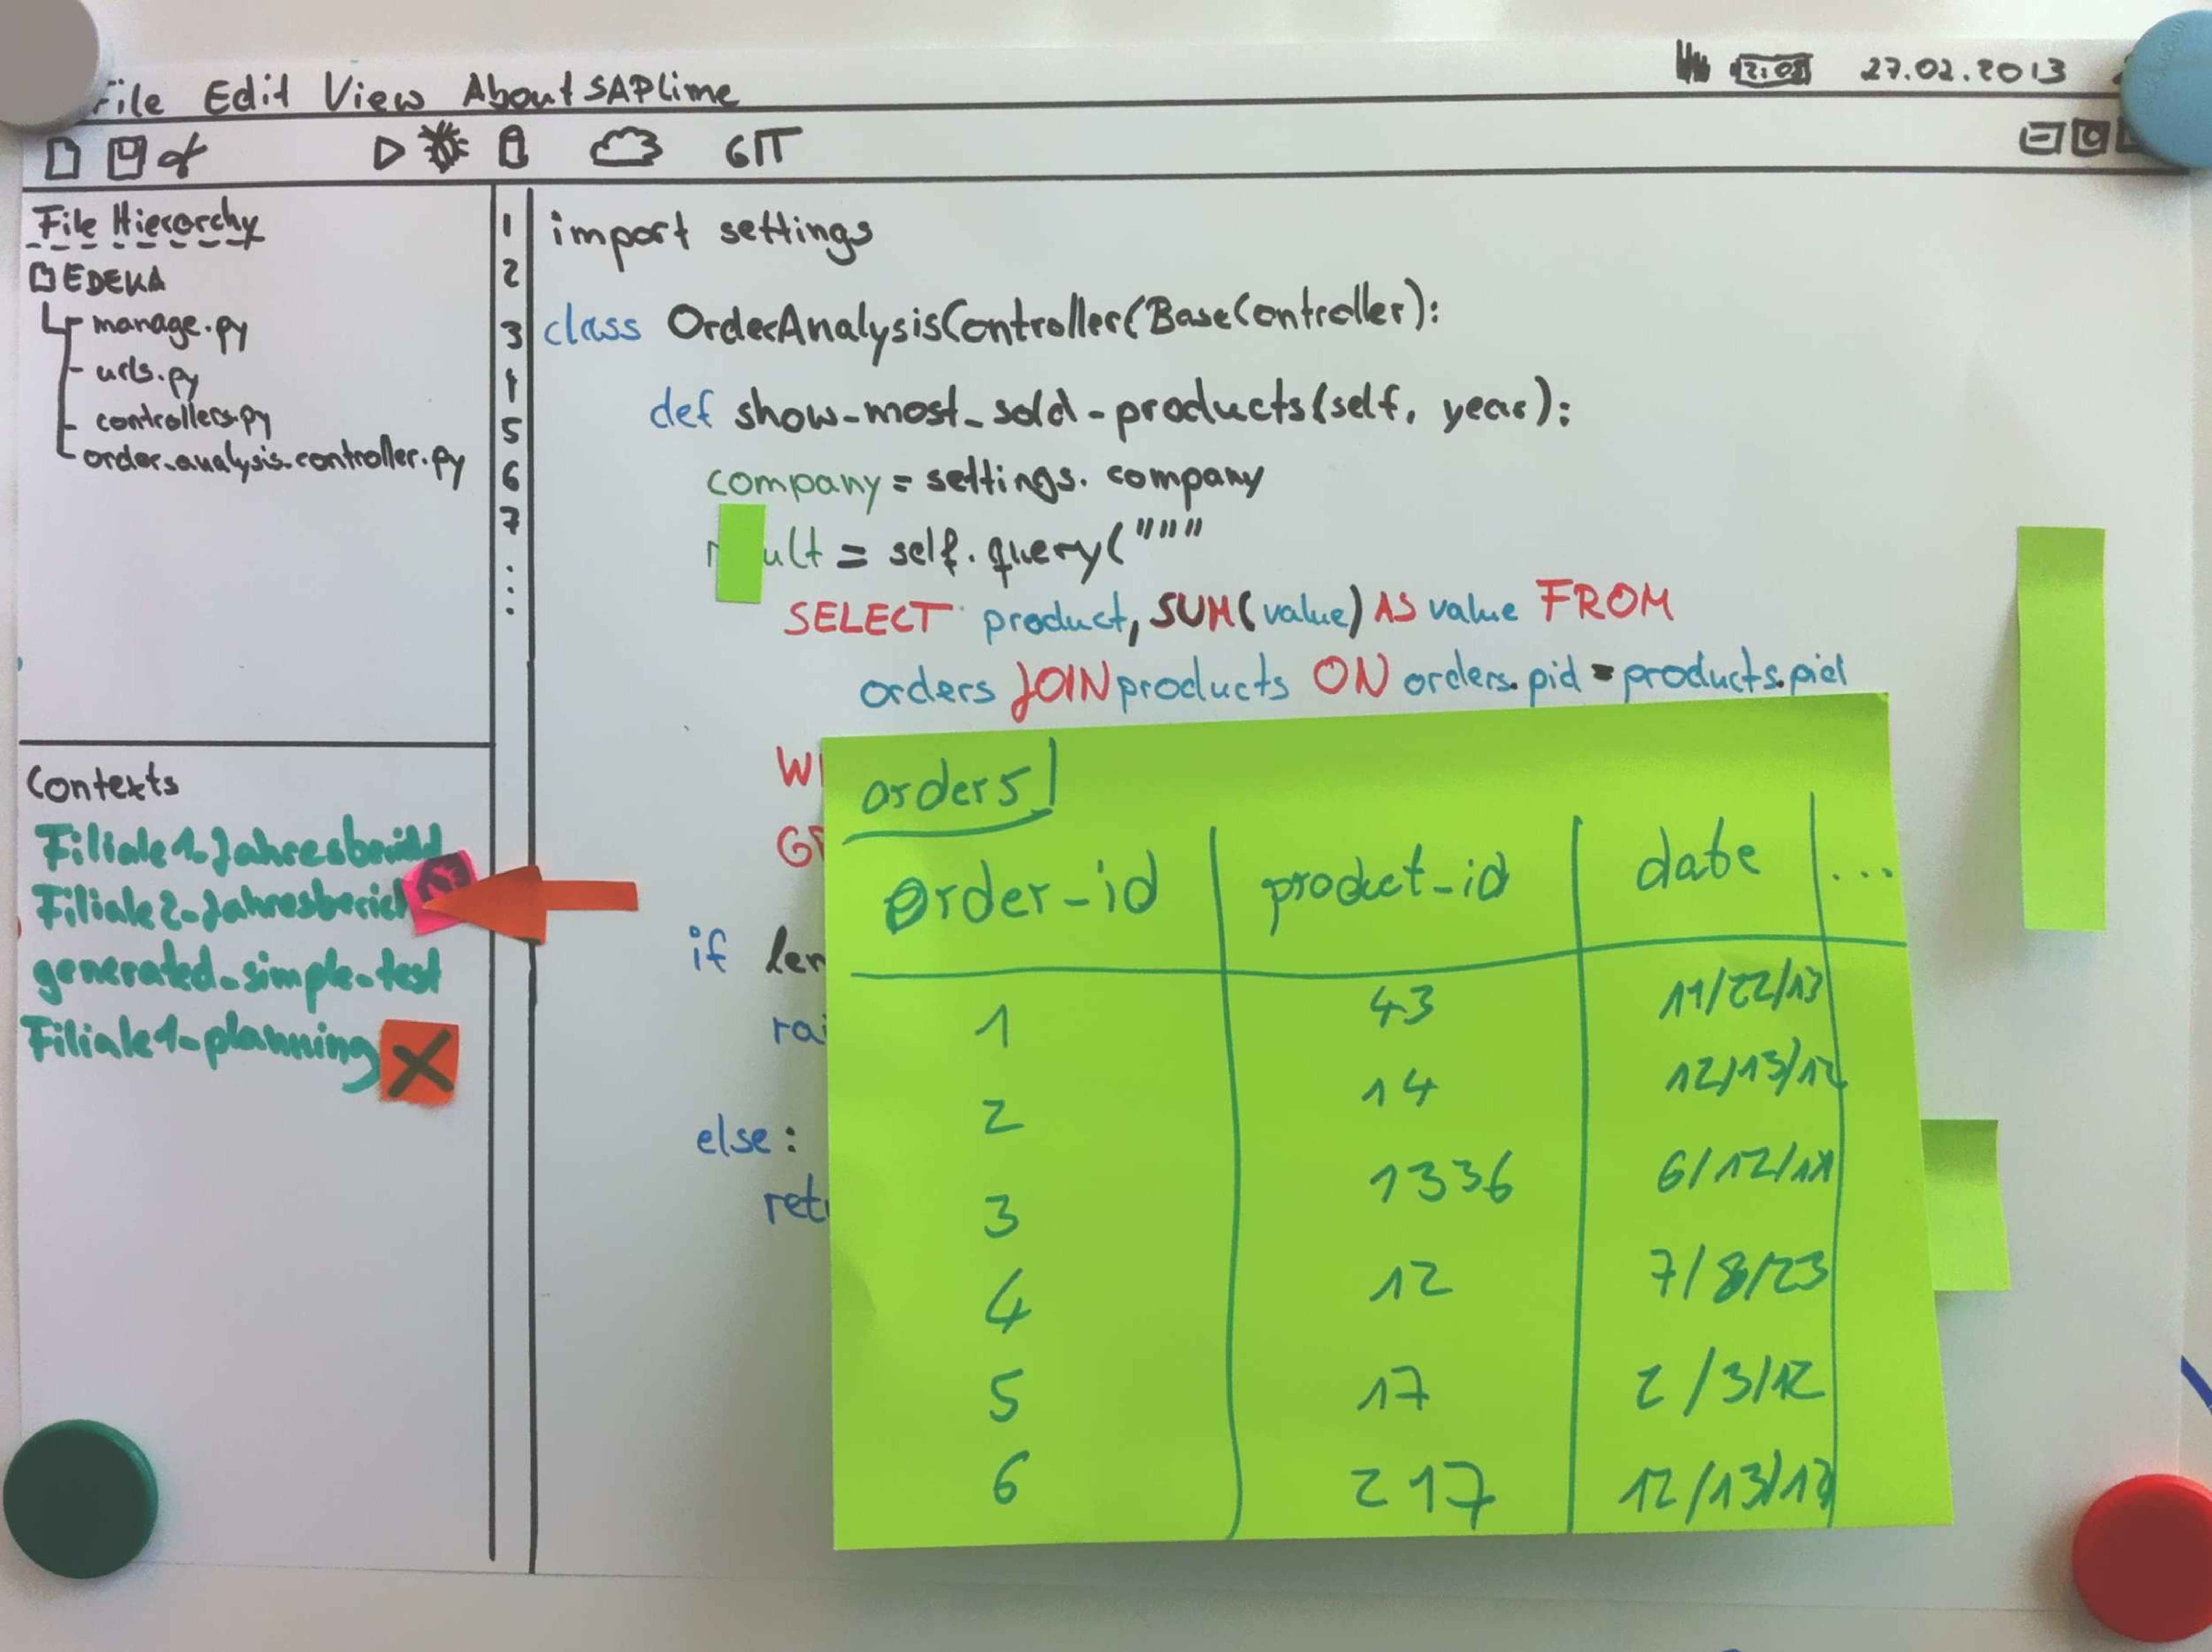
\includegraphics[width=0.8\linewidth]{images/paper_prototype2}
    \caption{Table Popup on our paper prototype after selecting the data table entity "orders."}
    % #selfrespect
    \label{fig:paper_prototype2}
\end{centering}
\end{figure}

From a DIN A3 format cardboard we tinkered a representation of our conceived code editor. (Figure \ref{fig:paper_prototype2})
It displays a piece of code in a \emph{Python}-inspired programming language with embedded SQL statements.
The editor features global syntax highlighting and, compared to conventional code editors, introduces a new panel in the lower left. The \emph{Data Context Panel} lists all possible Data Contexts for this particular function.\\

For the user testing sessions we prepared several Post-its to simulate highlighting, cursor positioning and popping up windows. 
As shown in Figure \ref{fig:paper_prototype2}, small red paper squares indicate either performance or functional problems in some of the Data Contexts. 
A small red arrow hints to the currently selected Data Context. The small green Post-it represents the cursor that the user can interact with. 
The green stripes on the right mark the control flow that the execution of the currently selected data context covers. \\

When the user moves the cursor onto the identifier of a table used in the SQL query, a popup is presented that provides relevant information on this table.
Figure \ref{fig:paper_prototype2} shows an example of these Post-it popups, when selecting the table \emph{"orders"}. 
For different tables and Data Contexts we prepared several Post-its with empty tables, too large tables, and single rows. The latter could be attached in case the user inserted a new row.\\

For our testing scenario we marked one of the contexts as erroneous and another as a performance bottleneck. 
The test person was intended to inspect the several tables and examine the performance bottleneck or the program error respectively.







